% -- Encoding UTF-8 without BOM
% -- XeLaTeX => PDF (BIBER)

\documentclass{cv-style}     % Add 'print' as an option into the square bracket to remove colours from this template for printing.

\setdefaultlanguage[variant=british]{english}
\sethyphenation[variant=british]{english}{} % Add words between the {} to avoid them to be cut

%----------------------------------------------------------------------------------------
%	Page layout
%----------------------------------------------------------------------------------------
\cvheadheight{3.5cm}
\cvasidewidth{4.7}
\cvasidevpos{3.5}
\cvmainwidth{11.5cm}
\geometry{left=6.4cm, top=2.5cm, right=1cm, bottom=1cm}

%----------------------------------------------------------------------------------------
%	Bibliography
%----------------------------------------------------------------------------------------
\usepackage[sectcntreset]{bibtopic}
\usepackage{natbib}
\bibliographystyle{bib/achemso_perso}
\AtBeginDocument{\nocite{achemso-control}}
%\setlength{\bibsep}{2pt plus 0.3ex}

%----------------------------------------------------------------------------------------
%	hyperlink setup
%----------------------------------------------------------------------------------------
\hypersetup{
    pdftitle=Resume \textbar{} Germain Vallverdu,%
    pdfauthor=Germain Vallverdu
}

%----------------------------------------------------------------------------------------
%	Setup las updated text
%----------------------------------------------------------------------------------------
%\lastupdated{Last Updated on \today}

%----------------------------------------------------------------------------------------
%	Add a few custom packages
%----------------------------------------------------------------------------------------
\usepackage{fontawesome}

\begin{document}

\header{Germain }{Vallverdu}{Associate Professor -- PhD in Chemical Physics}          % Your name

%----------------------------------------------------------------------------------------
%	SIDEBAR SECTION  -- In the aside, each new line forces a line break
%----------------------------------------------------------------------------------------

\begin{aside}
    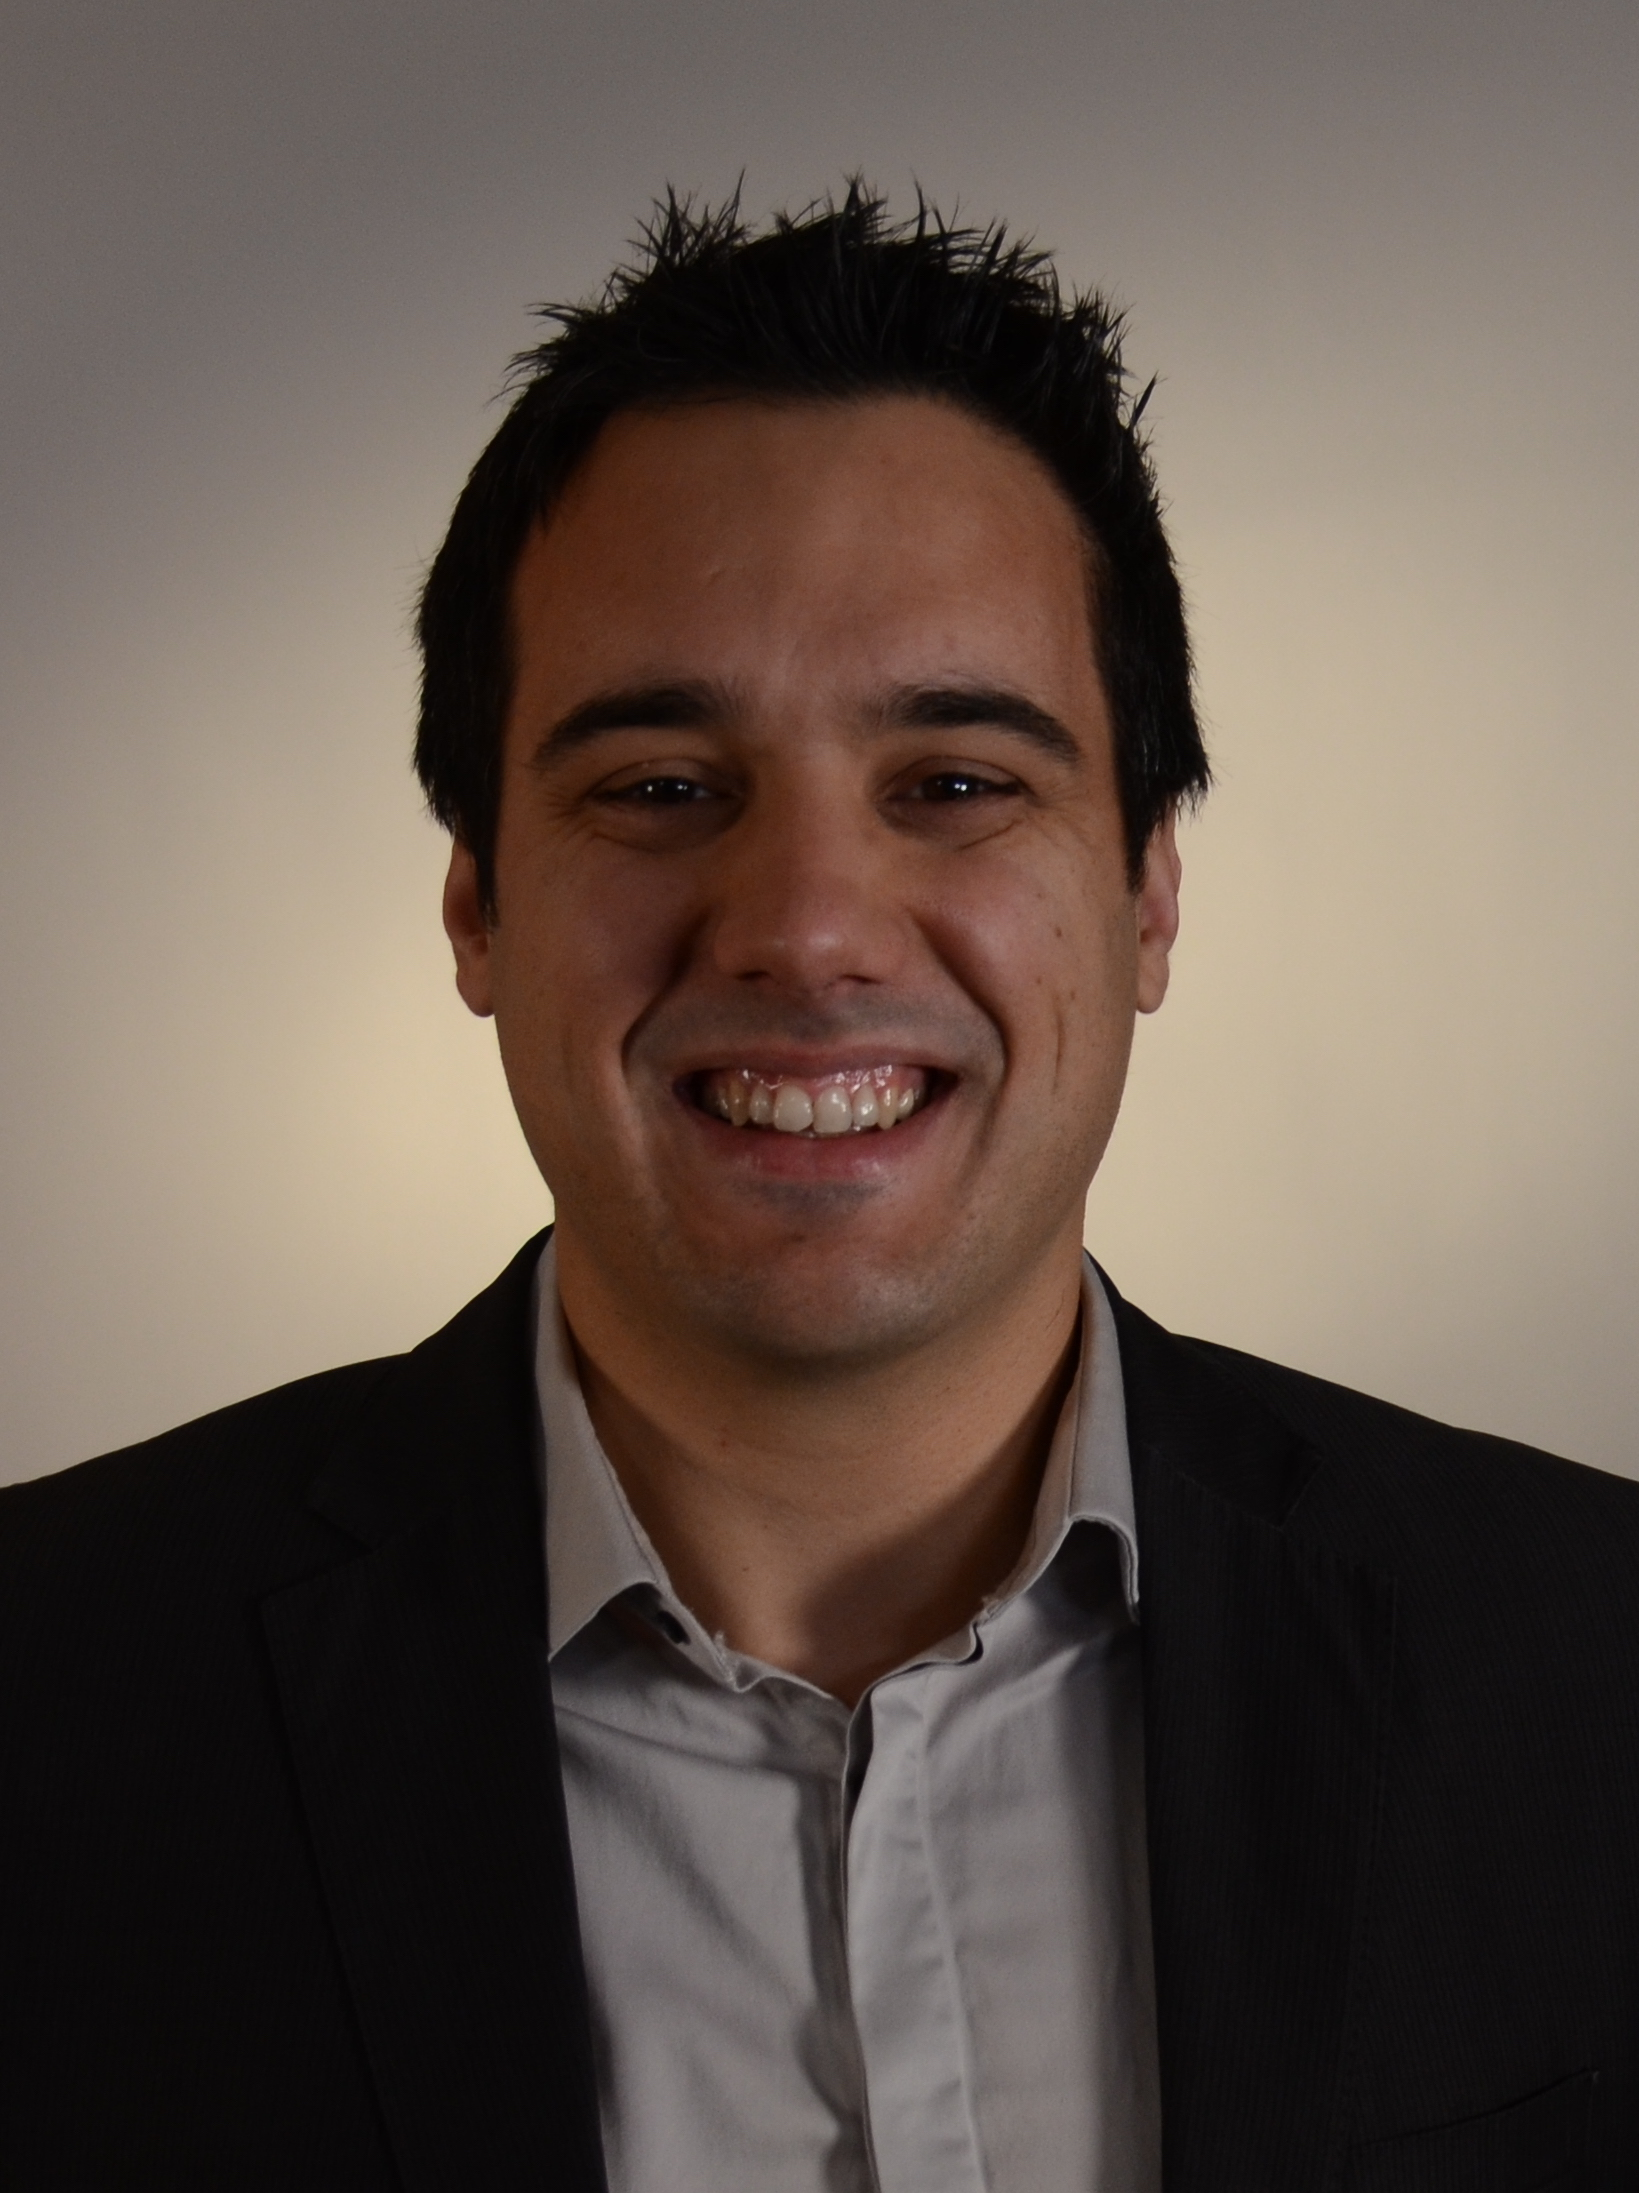
\includegraphics[width=.8\columnwidth]{img/gvallver}
    10 août 1983, France
    Maried, 2 children
    %
    \section{Contact}
    germain.vallverdu@univ-pau.fr
    (33) 5 59 40 78 51
    (33) 6 88 59 08 87
    ~
    IPREM
    Technopôle Hélioparc
    2 ave du Président P. Angot
    FR-64053 Pau cedex 9
    %
    \section{Theoretical Chemistry}
    Computational strategy
    Development
    Surfaces, interfaces
    VASP, CRYSTAL (solid)
    Gaussian (molecule)
    DL-POLY, AMBER (dynamic)
    %
    \section{Programming}
    Fortran, C
    Python
    \LaTeX{}, HTML/CSS
    %
    \section{Languages}
    French
    English (Professional)
    %
    \section{On the web}
    \href{http://orcid.org/0000-0003-1116-8776}{$\vcenter{\hbox{
\includegraphics{img/iD-icon}}}$ orcid.org/0000-0003-1116-8776}
    %\href{https://github.com/gVallverdu}{$\vcenter{\hbox{
\includegraphics[height=16pt]{img/GitHub-Mark}}}$ gVallverdu}
    \href{https://github.com/gVallverdu}{\faGithub{} gVallverdu}
    \href{http://gvallver.perso.univ-pau.fr}{\faGlobe{} gvallver.perso.univ-pau.fr}
    %
\end{aside}

\section{Abs}{tract}
\vspace{-0.2cm}

Assistant professor at the Université de Pau et des Pays de l'Adour,
I am a theoretical chemist at IPREM institute (Institute for Analytical sciences and
chemical physics applied to environment and materials).
My research activities concern the development of new methods and computational
strategies at different time or space scales, applied to the investigations
of complex systems.
I teach mainly chemical-physics subjects and programming languages at the university of Pau.

%----------------------------------------------------------------------------------------
%	SKILLS SECTION
%----------------------------------------------------------------------------------------

%\section{skills}
%  \vspace{-0.2cm}

%Skill 1, skill 2, skill 3, skill 4, skill 5.

%----------------------------------------------------------------------------------------
%	WORK EXPERIENCE SECTION
%----------------------------------------------------------------------------------------

\section{Professional }{Experiences}
\vspace{-0.2cm}

\begin{entrylist}
%------------------------------------------------
\entry
  {since 2010~}
  {Université de Pau et des Pays de l'Adour}
  {Pau, France}
  {\jobtitle{Associate professor}\\
   Theoretical chemistry and computational approaches.
   Surfaces, interfaces, reactivity and molecular interactions.}
%------------------------------------------------
\entry
  {2009--2010}
  {CEA - DAM}
  {Bruyères le châtel, France}
  {
  \jobtitle{Postdoctoral position}\\
  Development and implementation of a mesoscopic model for reactive shock waves
  propagation in heterogeneous systems.
  }
%------------------------------------------------
\entry
  {2006--2009}
  {Université Paris-Sud 11}
  {Orsay, France}
  {
  \jobtitle{PhD Student}\\
  Theoretical study of photophysical processes in fluorescent proteins.\\
  }
%------------------------------------------------
\end{entrylist}

%----------------------------------------------------------------------------------------
%	EDUCATION SECTION
%----------------------------------------------------------------------------------------
\vspace{-4mm}
\section{Educ}{ation}
\vspace{-0.2cm}

\begin{entrylist}
%------------------------------------------------
\entry
{2006-2009}
{PhD in chemistry {\normalfont speciality theoretical chemistry}}
{Université Paris-Sud 11}
{Mention très honorable}
%------------------------------------------------
\entry
{2004-2006}
{Master degree of chemistry}
{Université Paris-Sud 11}
{{\normalfont speciality molecular chemical-physics}\par Mention TB}
%------------------------------------------------
\entry
{2003-2004}
{Bachelor Degree of chemical-physics}
{Université Paris-Sud 11}
{Mention TB}
%------------------------------------------------
\entry
{2003-2006}
{Magistère de Physico-Chimie Moléculaire}
{Université Paris-Sud 11 -- ENS Cachan}
{\vspace{-4mm}}
%------------------------------------------------
\entry
{2001-2003}
{Undergraduate {\normalfont physics and chemistry}}
{Lycée François Arago, Perpignan}
{}
\end{entrylist}

%----------------------------------------------------------------------------------------
%	OTHER QUALIFICATIONS SECTION
%----------------------------------------------------------------------------------------
\vspace{-4mm}
\section{Main}{ publications}
\vspace{-0.2cm}
\nocite{aqturin2018_1, santos2017, vallverdu2016, guille2015, Martin2012, Maillet2011, Vallverdu2010}
\begin{btSect}{bib/articles}
    \btPrintCited
\end{btSect}

%----------------------------------------------------------------------------------------
%	INTERESTS SECTION
%----------------------------------------------------------------------------------------

% \section{interests}
%   \vspace{-0.2cm}
%
% \textbf{professional:} professional interest 1, professional interest 2 and professional interest 3.
% \textbf{personal:} personal interest 1, personal interest 2, personal interest 3 and personal interest 4.

%----------------------------------------------------------------------------------------
%	INTERESTS SECTION
%----------------------------------------------------------------------------------------

\section{Teach}{ing}
  \vspace{-0.2cm}

\begin{itemize}
    \item Lectures in chemical-physics, theoretical chemistry and programming languages, in bachelor
    degrees, master degrees and doctoral school.
    \item Science popularization: Quantum mechanics, animations for secondary and primary school pupils
\end{itemize}

%----------------------------------------------------------------------------------------

\end{document}
